\section{Results}
In this chapter, the aim is to:
\begin{itemize}
    \item Apply the objectives set out in the Testing Plan in Chapter 5
    \item Compare the performance of the five neural network architectures for cuffless estimation of blood pressure using PPG
    \item Assess whether the performance of the neural networks in estimating cuffless blood pressure meets the required standards set in the previous chapter 
\end{itemize}
\begin{comment}

\begin{itemize}
    \item An empirical relationship between
    parameters and results may be investigated,
    typically through the use of appropriate
    graphs.
    \item Where theory predicts aspects of
    performance the results can be compared
    with expectation and differences noted and (if
    possible) explained.
    \item Semi-empirical models of behaviour may be
    developed, justified, and tested.
    \item The types of experiments/simulations that
    were carried out should be described. Why
    were certain experiments carried out but not
    others? What were the important parameters
    in the simulation and how did they affect the
    results? 
\end{itemize}
\end{comment}



\subsection{Introduction}
This overview is split into five sections, one for each neural network architecture. Each section will contain the following: 
\begin{itemize}
    \item Mean Absolute Error (MAE) of the Systolic and Diastolic blood pressure against Epochs curves for the training set
    \item MAE of SBP and DBP against Epochs curves for the validation set
    \item The above two sets of curves with the addition of the first and second derivatives of the PPG signal with respect to time
    \item MAE table of results for all architectures 
    \item Training and inference times
\end{itemize}

\subsubsection{Introductory disclaimer}
The $4 \times 4$ subplots for the MAE are arranged in the following order:
\begin{itemize}
    \item Top-left curve: Mean Absolute Error (MAE) of Systolic blood pressure estimation using the training dataset, in mmHg, against the number of Epochs, in Arbitrary Units (AU)
    \item Top-right curve: MAE of Diastolic blood pressure estimation using the training dataset, in mmHg, against the number of Epochs
    \item Bottom-left curve: MAE of SBP estimation using the validation dataset against Epochs
    \item Bottom-right curve: MAE of DBP estimation using the validation dataset against Epochs
\end{itemize}

\subsection{AlexNet}
Figure \ref{alexnetResults} shows the performance of the AlexNet architecture using only the PPG segmented windows. 
As illustrated below, the two training curves show a very significant drop in MAE after approximately 5 Epochs in training, indicating 
that the model has learned the patterns of the training data well. Regarding the two validation curves, despite there being a 
significant low MAE for approximately 50 Epochs of testing, there are noticeable spikes in MAE occuring during the remaining 50 Epochs.
\begin{figure}[H]
    \centering
    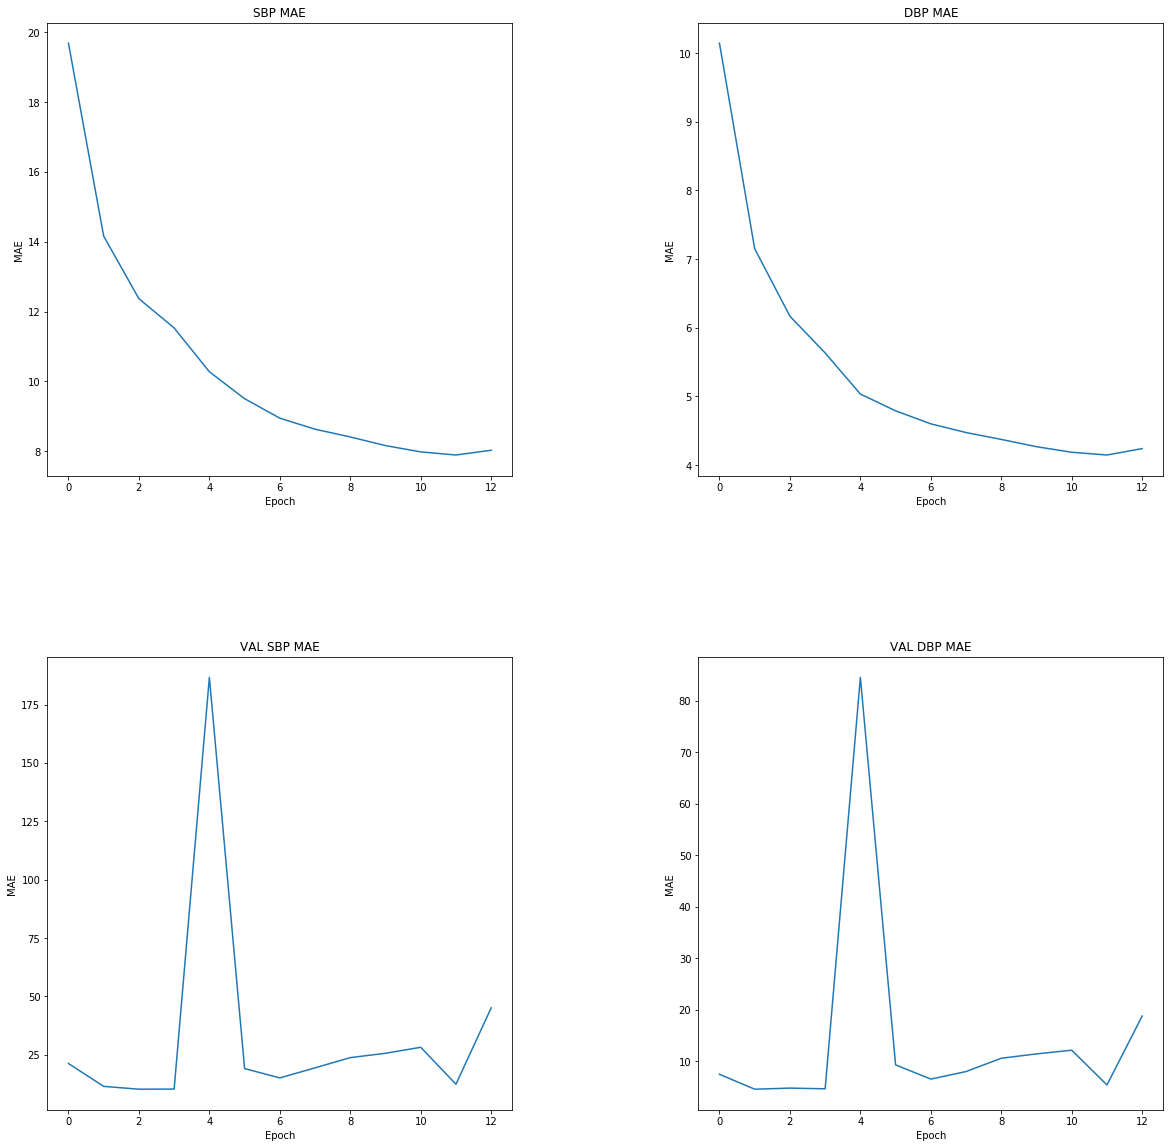
\includegraphics[width=15cm,height=15cm,keepaspectratio]{Results/alexnet.png}
    \caption{MAE of SBP and DBP for the AlexNet architecture}
    \label{alexnetResults}
\end{figure}\noindent Figure \ref{alexnetDerivResults} illustrates the same training and validation 
curves with the addition of the first and second derivatives of the PPG signal. This model also performs 
well on the training data, but also appears to have a better quality of estimation on the validation dataset, due to the lack 
of noticeable upward spikes in the MAE.
\begin{figure}[H]
    \centering
    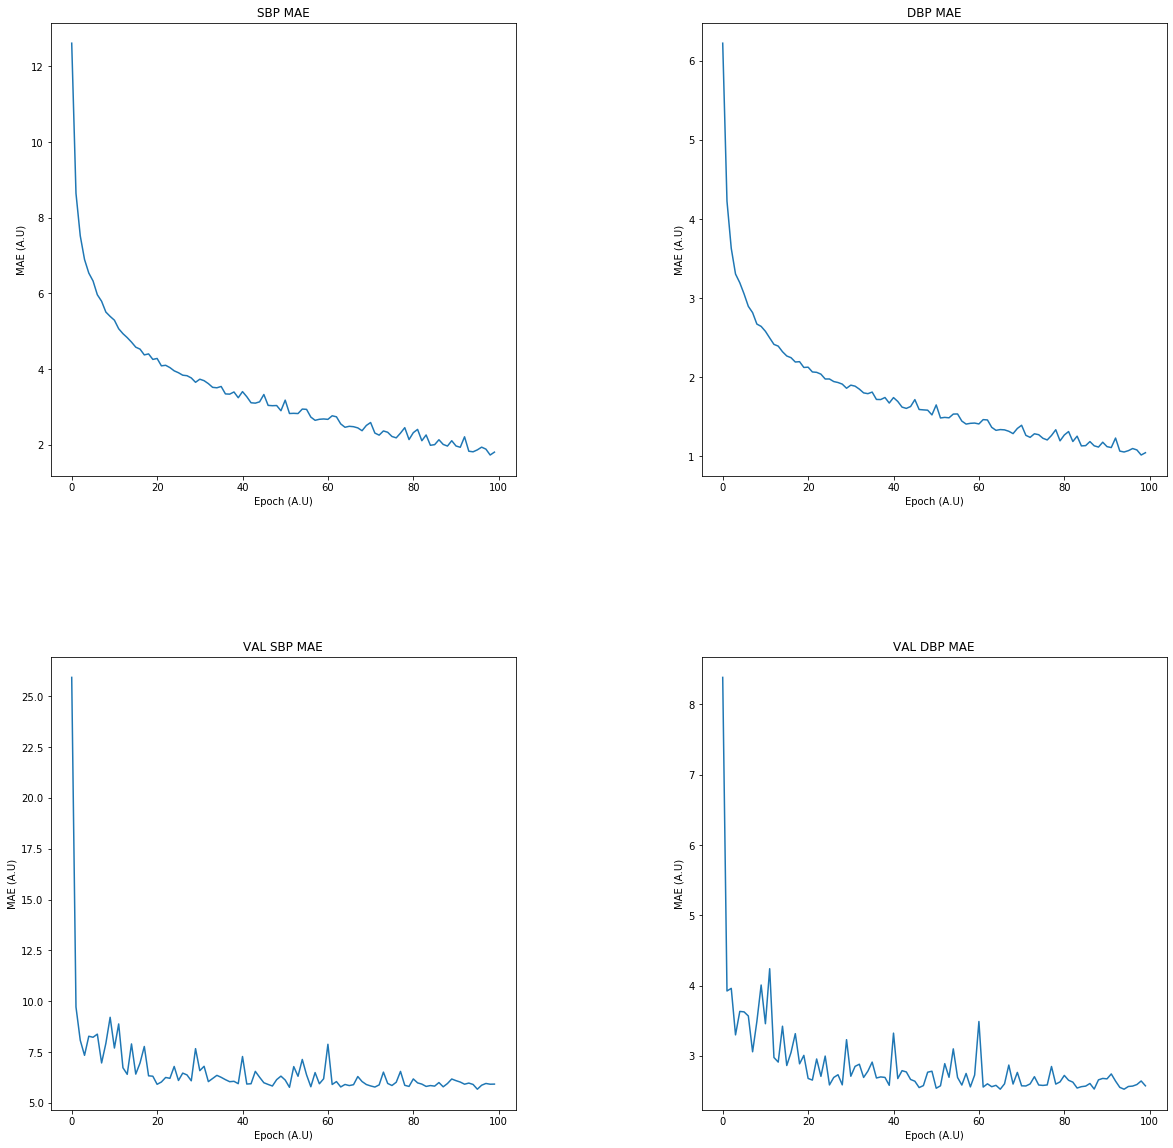
\includegraphics[width=15cm,height=15cm,keepaspectratio]{Results/resnetDeriv.png}
    \caption{MAE of SBP and DBP for the AlexNet architecture with the PPG derivative features}
    \label{alexnetDerivResults}
\end{figure}

\subsection{ResNet}
Figure \ref{resnetResults} shows the performance of the ResNet architecture using only the PPG segmented windows. 
As illustrated below, the two training curves show a steady drop in MAE throughout the training process, indicating 
that the model has learned the patterns of the training data well. There are similar noticeable upward spikes in the validation curves, 
suggesting that this is a linking factor between the performance of CNN architectures on this particular dataset.
\begin{figure}[H]
    \centering
    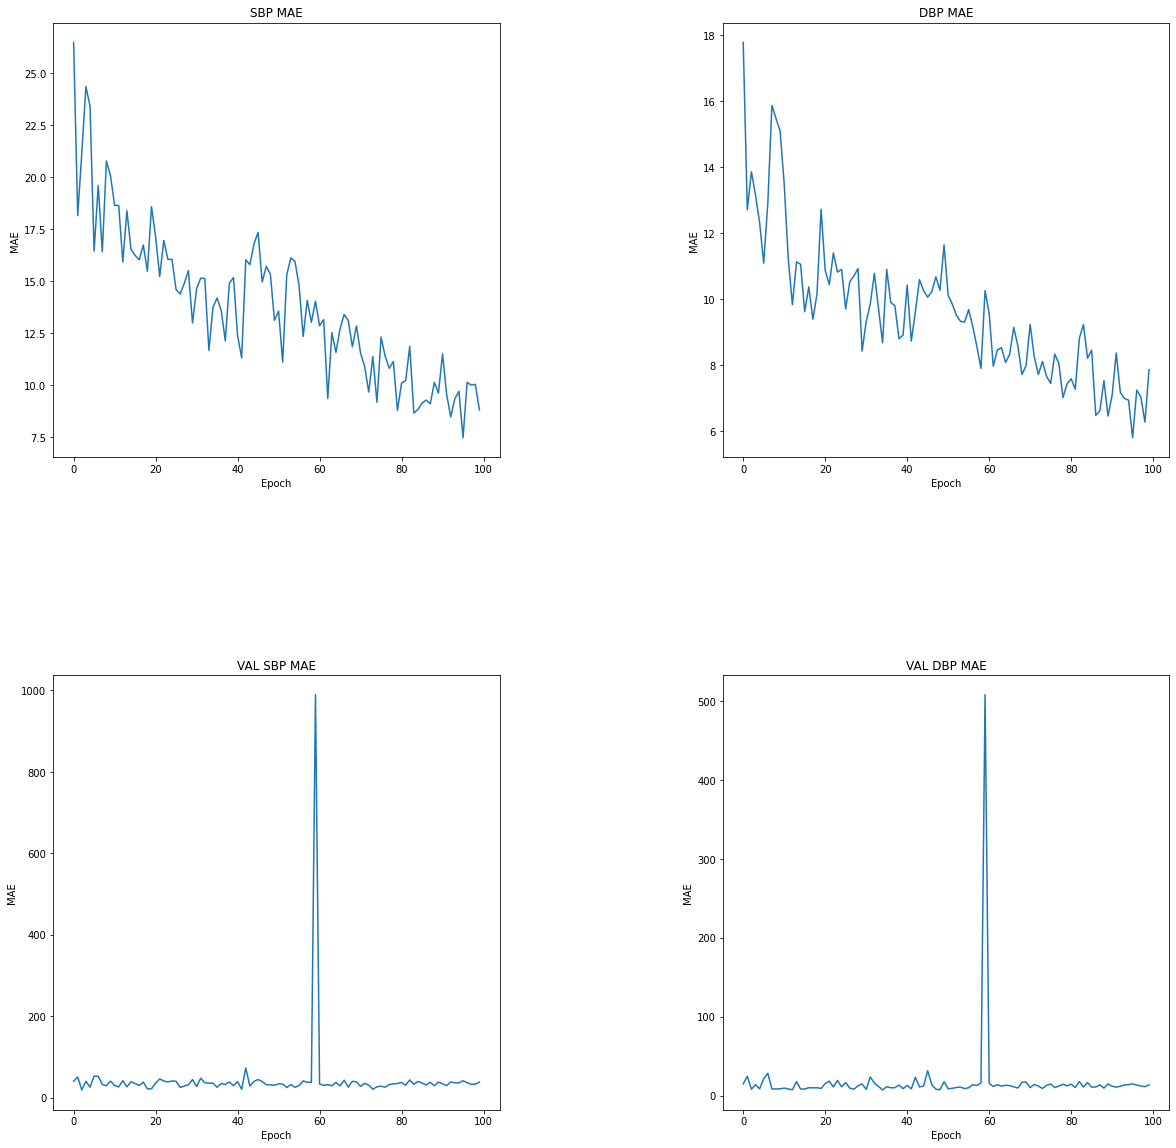
\includegraphics[width=15cm,height=15cm,keepaspectratio]{Results/resnet.png}
    \caption{MAE of SBP and DBP for the ResNet architecture}
    \label{resnetResults}
\end{figure}\noindent Figure \ref{resnetDerivResults} illustrates the same training and validation 
curves with the addition of the first and second derivatives of the PPG signal. This model appears to perform better on the training 
data than the previous model, as there is less variation in the MAE curves for increasing Epochs. 
well on the training data. There is also a better quality of estimation on the validation dataset, due to both the sudden drop in MAE after approximately 
4 Epochs and the lack of noticeable upward spikes in the MAE.
\begin{figure}[H]
    \centering
    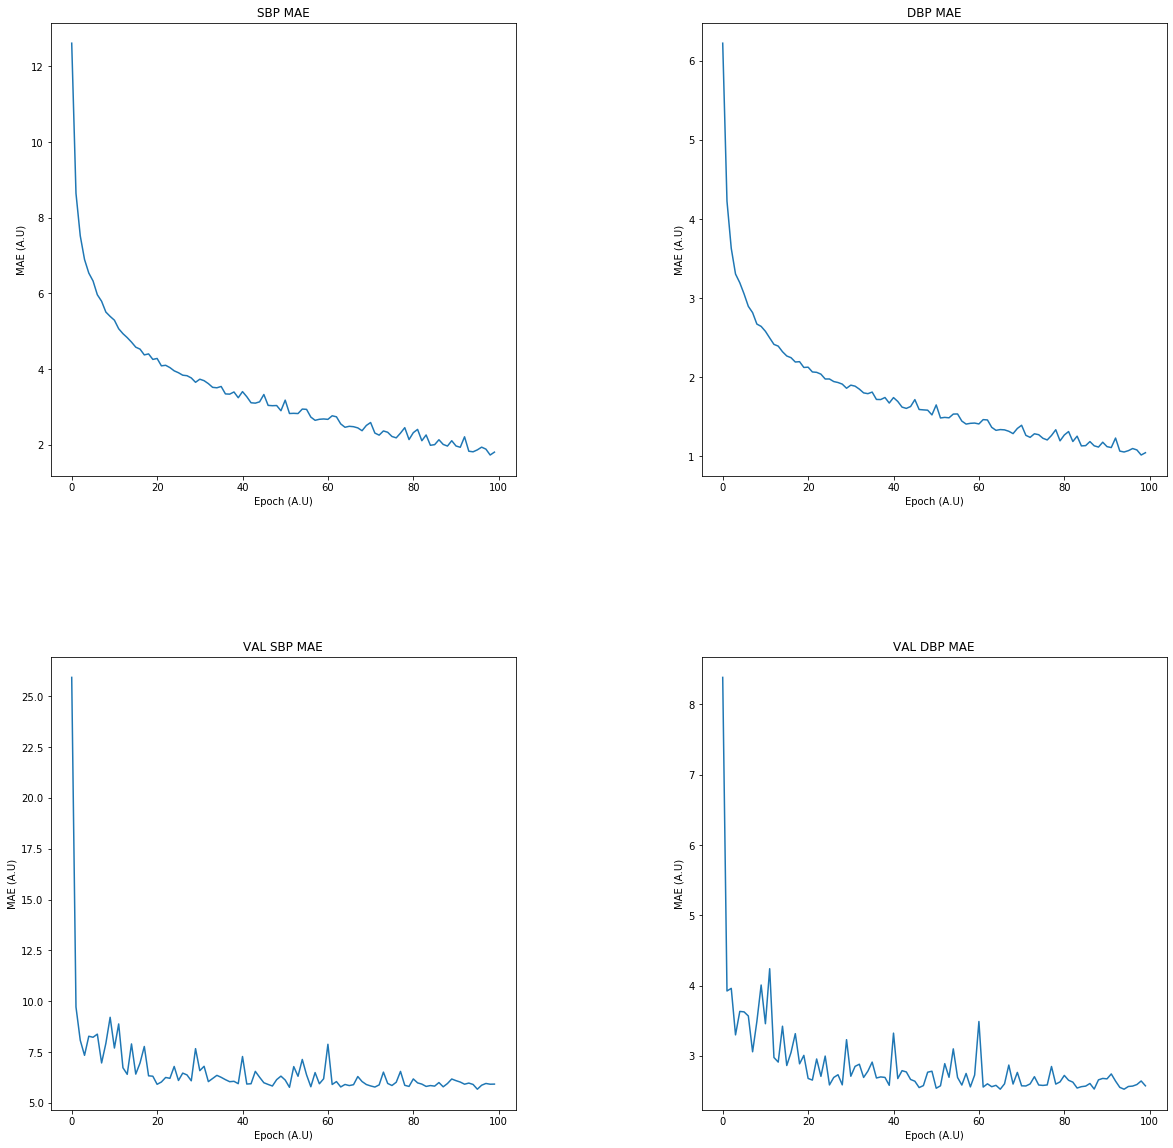
\includegraphics[width=15cm,height=15cm,keepaspectratio]{Results/resnetDeriv.png}
    \caption{MAE of SBP and DBP for the ResNet architecture with the PPG derivative features}
    \label{resnetDerivResults}
\end{figure}

\subsection{ResNet with LOSO}
Figure \ref{resnetLosoResults} shows the performance of the ResNet-LOSO architecture using only the PPG segmented windows. 
As illustrated below, the two training curves show a steady drop in MAE throughout the training process, indicating 
that the model has learned the patterns of the training data well. There is now a reduction in the upward spikes in the validation 
curves, indicating that the implementation of an architecture that is both a function of frequency and time (or spectro-temporal architecture) is beneficial, 
as there are now more features available for extraction during each PPG window segment.
\begin{figure}[H]
    \centering
    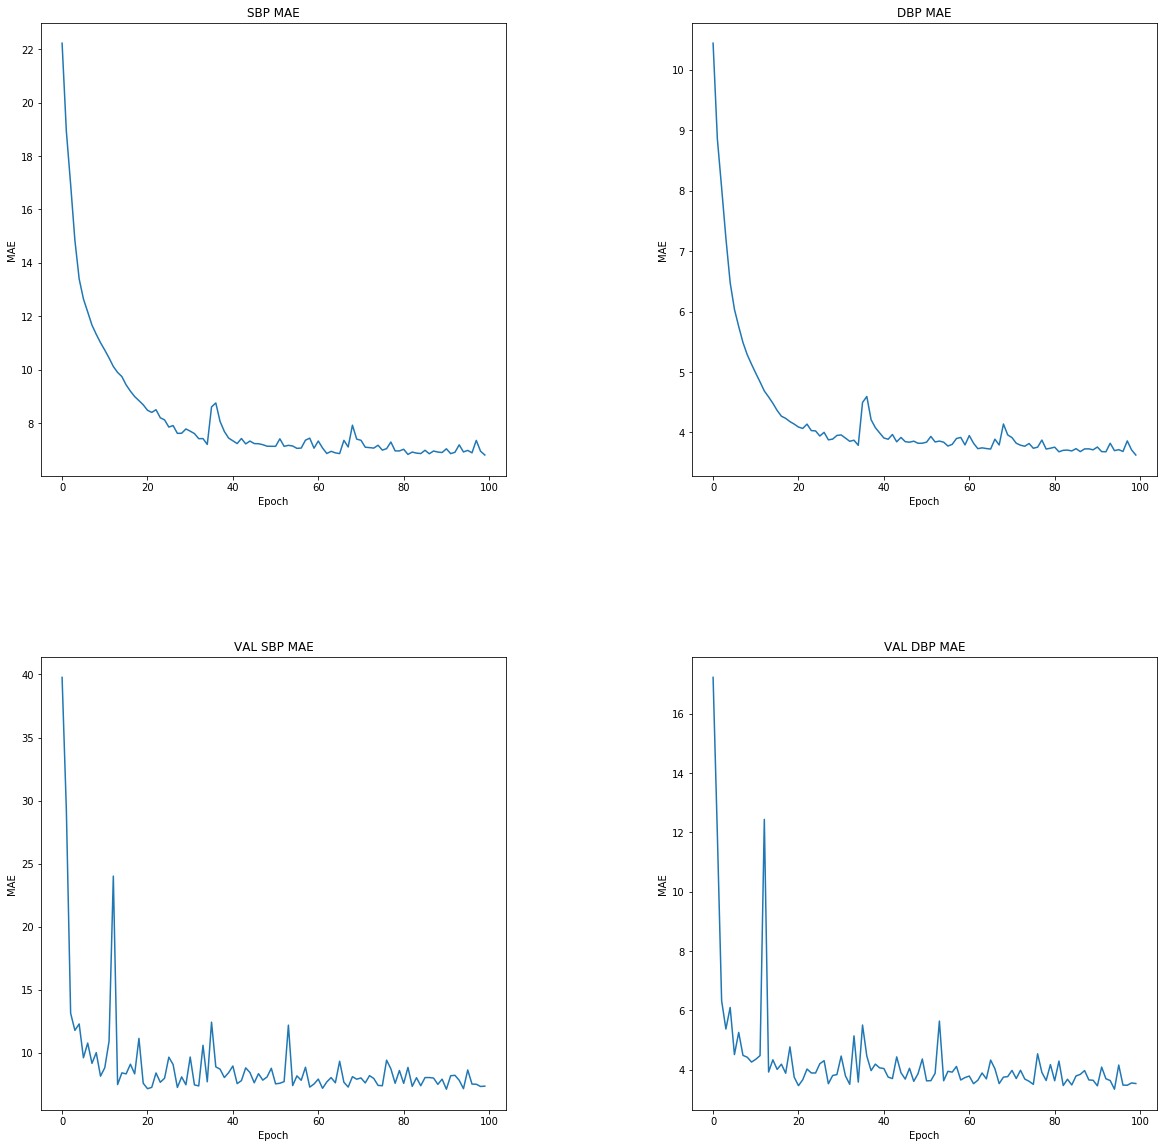
\includegraphics[width=15cm,height=15cm,keepaspectratio]{Results/slapnicar.png}
    \caption{MAE of SBP and DBP for the ResNet-LOSO architecture}
    \label{resnetLosoResults}
\end{figure}\noindent Figure \ref{resnetLosoDerivResults} indicates that the performances of all curves 
are in fact very similar to the implementation without the additional PPG features. This suggests that 
the base ResNet-LOSO architecture has sufficient capabilities to automatically extract PPG features during 
each segmented window.
\begin{figure}[H]
    \centering
    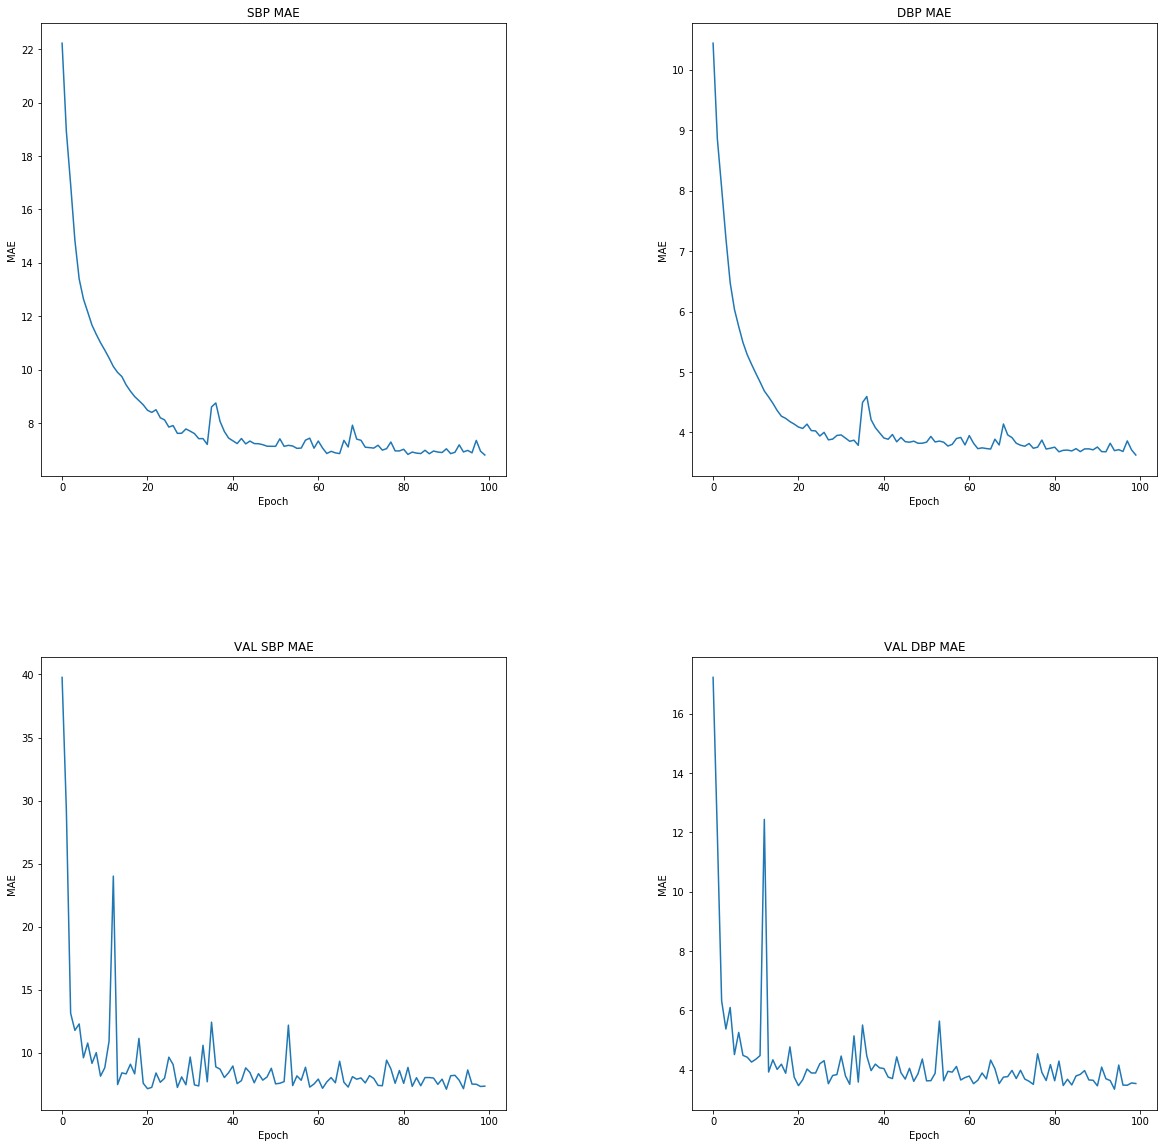
\includegraphics[width=15cm,height=15cm,keepaspectratio]{Results/slapnicar.png}
    \caption{MAE of SBP and DBP for the ResNet-LOSO architecture with the PPG derivative features}
    \label{resnetLosoDerivResults}
\end{figure}


\subsection{Bi-directional LSTM}
Figure \ref{lstmResults} shows the performance of the Bi-directional LSTM architecture using only the PPG segmented windows. 
It is clear that the training curves do not perform as well on the training and validation data compared to the 3 previous CNN architectures, due to the volatile 
nature of all four curves.
\begin{figure}[H]
    \centering
    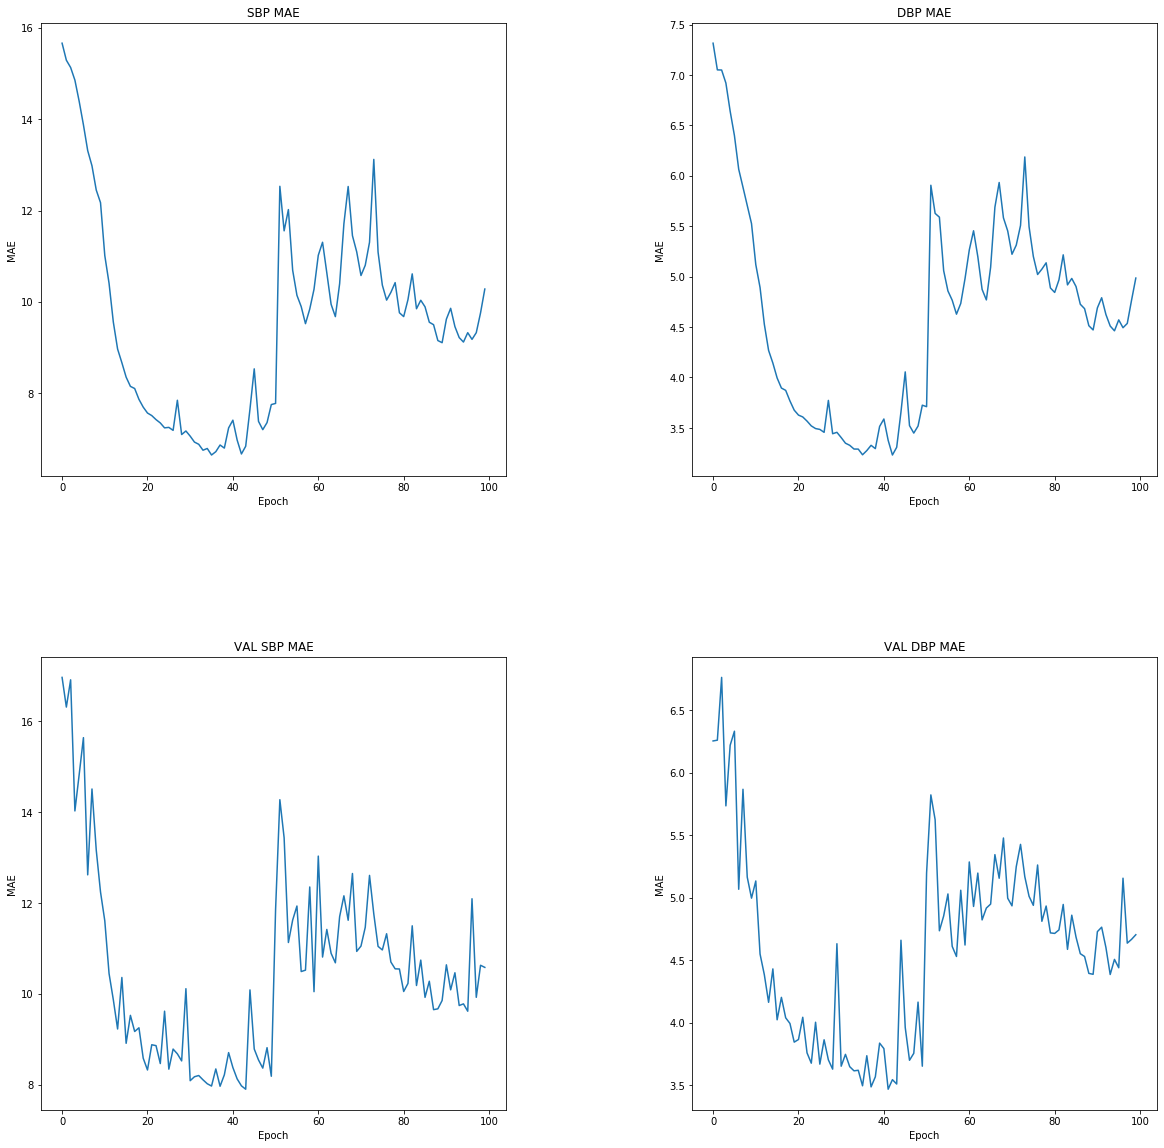
\includegraphics[width=15cm,height=15cm,keepaspectratio]{Results/lstm.png}
    \caption{MAE of SBP and DBP for the LSTM architecture}
    \label{lstmResults}
\end{figure}\noindent Figure \ref{lstmDerivResults} shows that the addition of the PPG 
features does appear to smoothen the training curves, however it still does not have 
any significant effect on the validation curves.
\begin{figure}[H]
    \centering
    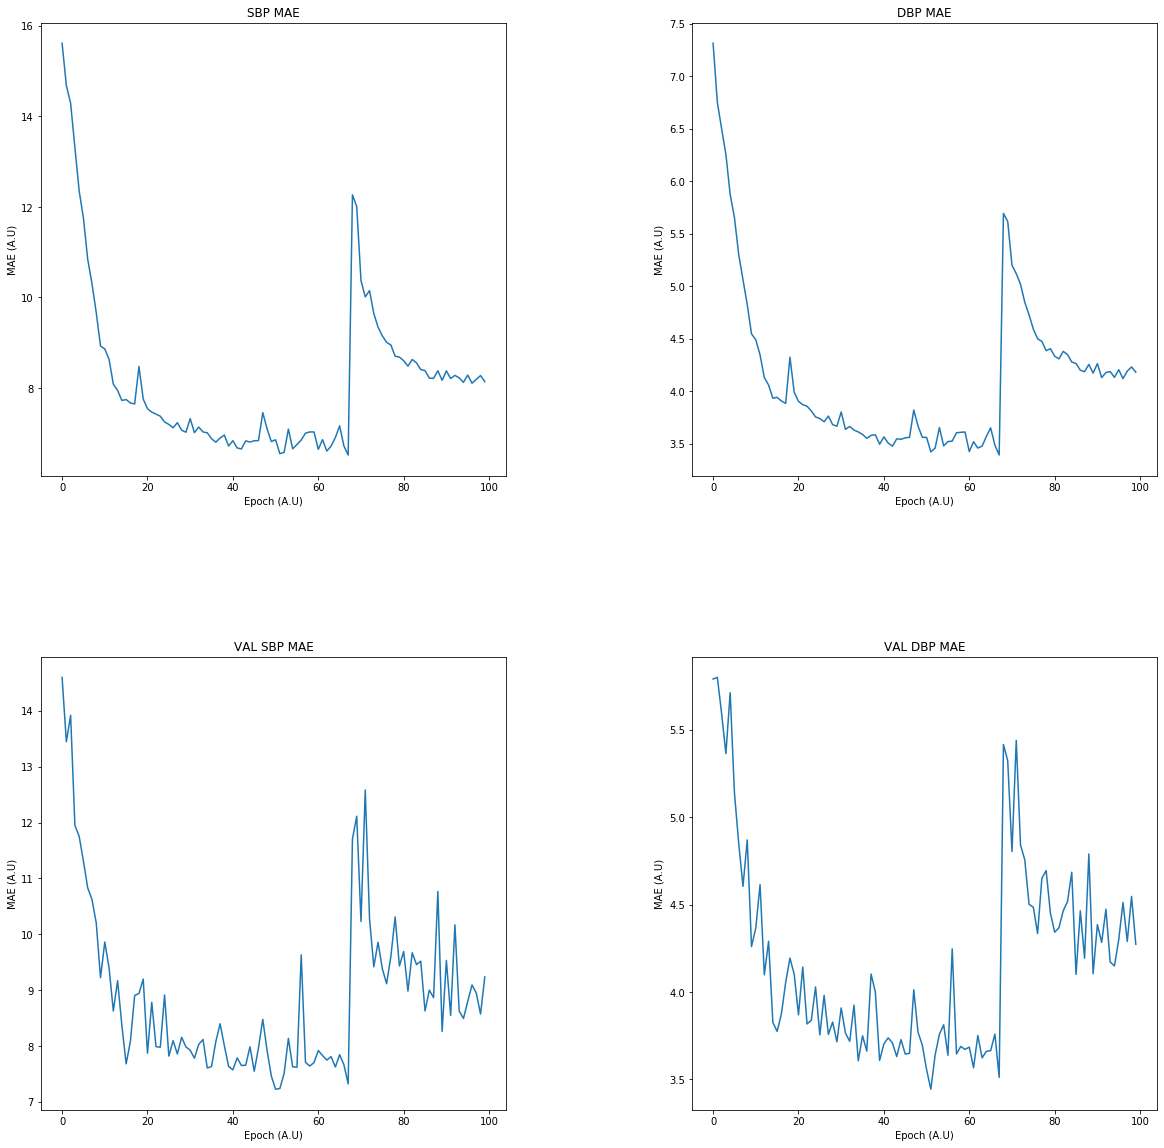
\includegraphics[width=15cm,height=15cm,keepaspectratio]{Results/lstmDeriv.png}
    \caption{MAE of SBP and DBP for the LSTM architecture with the PPG derivative features}
    \label{lstmDerivResults}
\end{figure}

\subsection{Transformer Encoder}
Figure \ref{encoderResults} shows the performance of the Transformer encoder architecture using only the PPG segmented windows. 
It is clear that the model has acceptable performance on the training dataset, due to the steady reduction in the MAE curves 
for increasing Epochs. However, for the validation dataset, although there is a gradual decrease in the MAE estimation, there is a lot 
of variance in the MAE for increasing Epochs.
\begin{figure}[H]
    \centering
    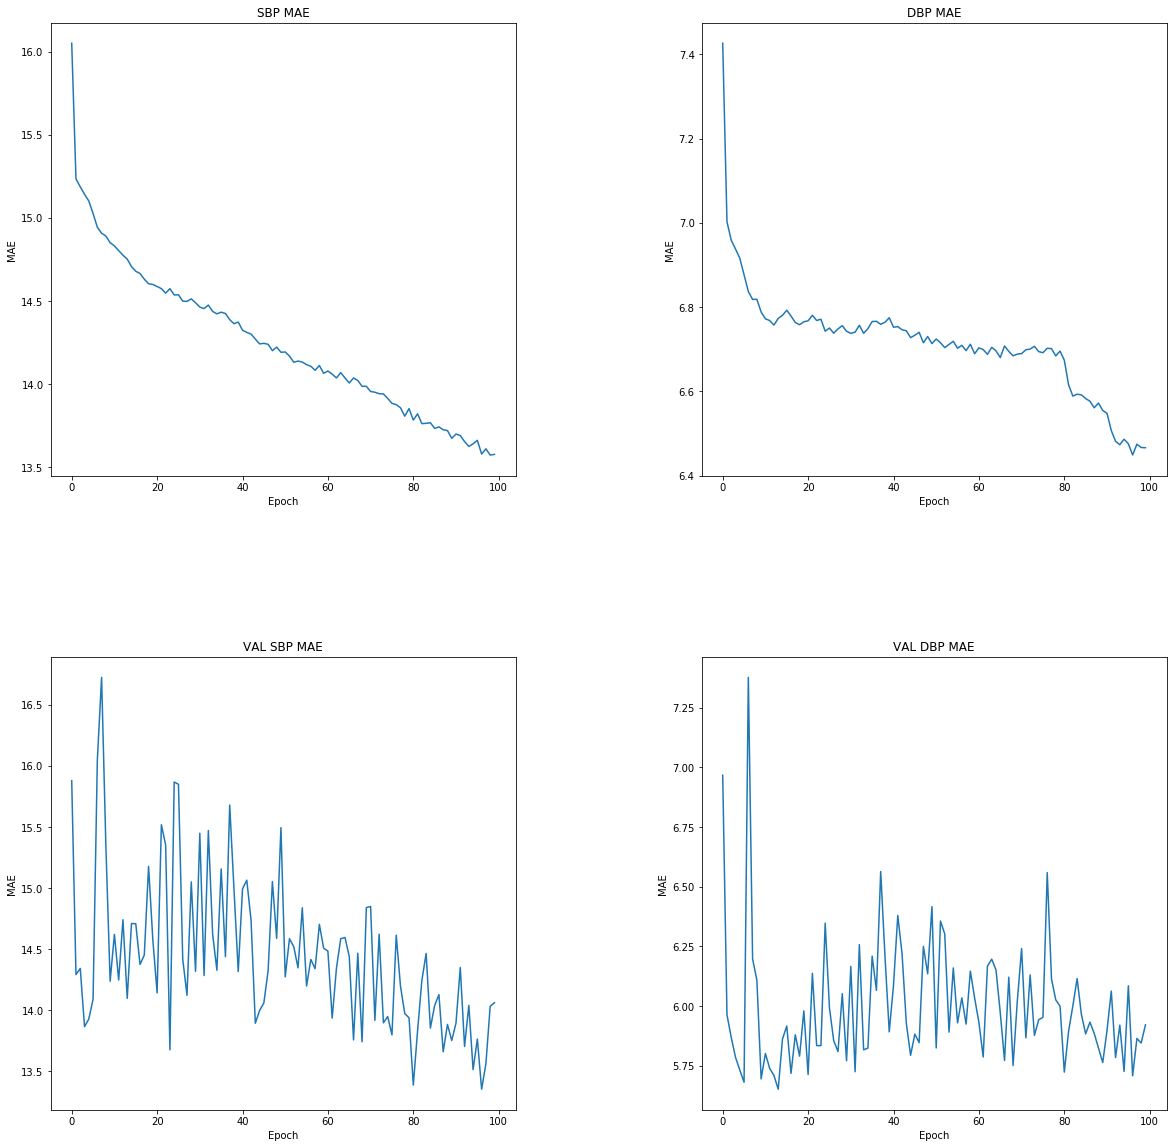
\includegraphics[width=15cm,height=15cm,keepaspectratio]{Results/encoder.png}
    \caption{MAE of SBP and DBP for the Transformer encoder architecture}
    \label{encoderResults}
\end{figure}\noindent Figure \ref{encoderDerivResults} does indicate an improvement in the training curves, suggesting 
that it is beneficial to add the PPG derivative features to the model's input. However, there is still very minimal 
change in the validation curves.
\begin{figure}[H]
    \centering
    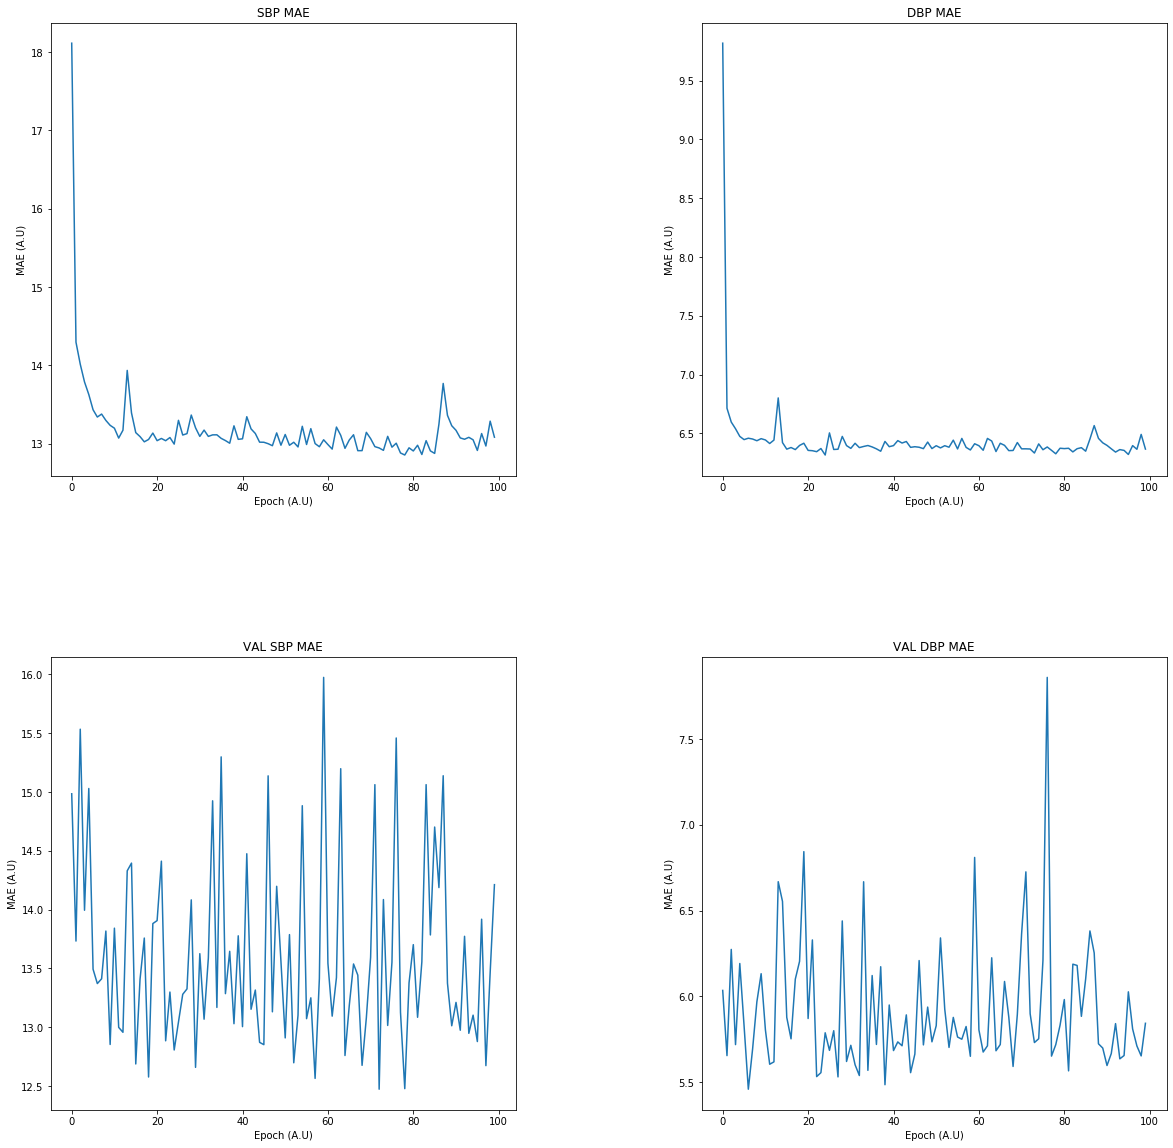
\includegraphics[width=15cm,height=15cm,keepaspectratio]{Results/encoderDeriv.png}
    \caption{MAE of SBP and DBP for the Transformer encoder architecture with the PPG derivative features}
    \label{encoderDerivResults}
\end{figure}

\subsection{Table of MAE results}
Based on Figures \ref{alexnetResults} to \ref{encoderDerivResults}, Table \ref{tabMaeResults} summarises the performances of each of the five neural 
network architectures and illustrates the effect of the addition of the PPG derivative features.
\begin{table}[H]
    \centering
    \caption{Minimum MAE of the five neural network architectures (average after running each configuration 3 times)}
    \label{tabMaeResults}
    \resizebox{\columnwidth}{!}{%
    \begin{tabular}{|c|cc|cc|}
    \hline
    \multirow{2}{*}{\textbf{Neural network architecture}} & \multicolumn{2}{c|}{\textbf{SBP MAE (mmHg)}} & \multicolumn{2}{c|}{\textbf{DBP MAE (mmHg)}} \\
                                                          & \textbf{Training}    & \textbf{Validation}   & \textbf{Training}    & \textbf{Validation}   \\ \hline
    AlexNet                             & 4.5867 & 4.6724 & 3.5892 & 3.7895 \\
    AlexNet with derivative             & 2.0134 & 6.7865 & 1.3424 & 2.9451 \\
    ResNet                              & 7.7123 & 9.8753 & 6.0123 & 10.297 \\
    ResNet with derivative              & 1.9845 & 6.9732 & 1.2765 & 2.2145 \\
    ResNet-LOSO                         & 7.5329 & 9.4234 & 4.2154 & 4.3785 \\
    ResNet-LOSO with derivative         & 7.4923 & 9.5246 & 3.7894 & 3.9720 \\
    LSTM                                & 5.1370 & 8.2793 & 3.2159 & 3.4196 \\
    LSTM with derivative                & 5.1299 & 8.2432 & 3.7913 & 3.5217 \\
    Transformer Encoder                 & 13.214 & 13.359 & 6.3412 & 5.6129 \\
    Transformer Encoder with derivative & 12.992 & 12.740 & 6.4387 & 5.4763 \\ \hline
    \end{tabular}%
    }
    \end{table}

\subsection{Training and Inference times}
As discussed previously in Chapter 2, the inference time is the time taken for any of the five 
neural network models to perform a prediction on the unseen test data. This time measurement 
is also a good indicator of how much depth, or how much complexity, a neural network architecture has. 
The inference time calculation was implemented using the following Python code,
\begin{figure}[H]
    \begin{python}
    import time
    # firstly iterate through each test sample
    for i in range(int(Ntest//batch_size)):
        # acquire the unseen test data sample with the .next() function
        ppg_test, BP_true = test_dataset.next()
        start_time = time.time()
        # apply the neural network model to the unseen data sample
        BP_est = model.predict(ppg_test)
        time_elapsed = time.time() - start_time
        print('Average inference time per test sample: {:.4f} (ms)'.format(1000*time_elapsed/len(ppg_test)))
\end{python}
\caption{Python code for finding the inference time}
\end{figure}\noindent In addition, the training times are displayed through the Python Tensorflow console interface and an average value can be calculated as a result. 
Hence, these times are displayed in Table \ref{tabTrainInfTimes}.
% Please add the following required packages to your document preamble:
% \usepackage{multirow}
% \usepackage{graphicx}
\begin{table}[H]
    \centering
    \caption{Average Training Times and Inference Times for the five neural network architectures (average after running each configuration 3 times)}
    \label{tabTrainInfTimes}
    \resizebox{\columnwidth}{!}{%
    \begin{tabular}{|c|cc|cc|}
    \hline
    \multirow{2}{*}{\textbf{Neural network architecture}} &
      \multicolumn{2}{c|}{\textbf{Average Training time (seconds per epoch)}} &
      \multicolumn{2}{c|}{\textbf{Average Inference Time (milliseconds per test sample)}} \\
     &
      \textbf{Without derivative features} &
      \textbf{With derivative features} &
      \textbf{Without derivative features} &
      \textbf{With derivative features} \\ \hline
    AlexNet             & 26.29  & 27.12  & \multicolumn{2}{c|}{0.5204} \\
    ResNet              & 130.49 & 130.12 & \multicolumn{2}{c|}{0.5756} \\
    ResNet-LOSO         & 59.04  & 126.27 & \multicolumn{2}{c|}{0.5891} \\
    LSTM                & 86.47  & 87.89  & \multicolumn{2}{c|}{0.6043} \\
    Transformer Encoder & 49.35  & 52.90  & \multicolumn{2}{c|}{0.3590} \\ \hline
    \end{tabular}%
    }
    \end{table}